\chapter{Simulation}
This section of the report describes the testing of separate signal processing steps in a simulated environment. Each block as seen in figure \ref{fig:global_thesis_flowchart} will be tested individually, and the method and results will be discussion on a per-block basis:
\begin{itemize}
    \item Pre-whitening
    \item Filtering
    \item Envelope estimation
\end{itemize}

Unless specified otherwise
\begin{itemize}
    \item all signals will be high-passed with a cutoff frequency of \SI{1}{\hertz} to remove DC bias before any operation is applied
    \item all measured sEMG signals were acquired during isometric contraction
\end{itemize}

\section{Pre-whitening}
A whitening filter is a digital filter with a frequency response that is (ideally) the inverse of the frequency contents of an sEMG signal. 

\subsection{Method}
A testing signal was created that approximates the frequency response of an sEMG signal. The testing signal was created by creating a long white noise signal and multiplying the amplitudes in the frequency spectrum with a curve that estimates the frequency response of an sEMG signal. After this the signal is passed through inverse fft to go back to a time-domain signal. The result can be seen in \ref{fig:whitening_simulation} subplot 1 and 2.

The whitening filter is then created by taking the FFT of the time-domain test signal and taking its reciprocal at every frequency. Lastly the whitening filter frequencies are multiplied by the mean of the original signal frequencies to make sure that when the filter is applied the mean stays the same. These steps can be seen in \ref{fig:whitening_simulation} subplot 3. 

\subsection{Results}
\begin{figure}[h!t]
	\begin{center}
		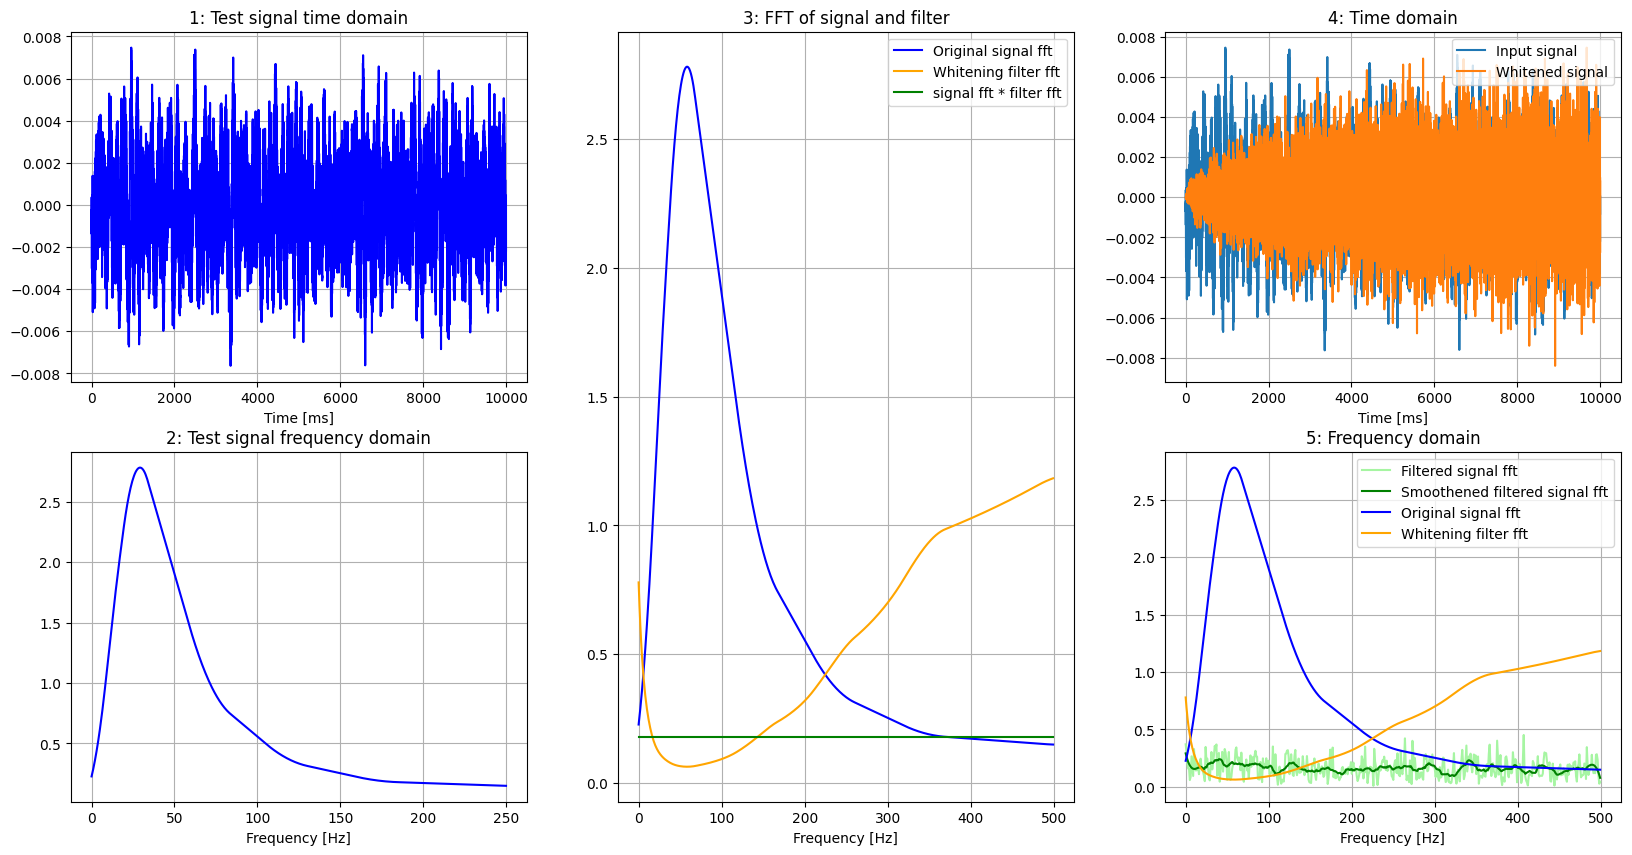
\includegraphics[width=1.0\columnwidth]{images/prewhitening_simulation.png}
	\end{center}
	\caption{Subplot 1 and 2 display the input simulated input signal with a frequency response that approximates the frequency contents of an sEMG signal. Subplot 3 displays the frequency content of the signal, the subsequently calculated whitening filter, and the multiplication of the signal with the filter in frequency domain to show that the response is indeed white. Subplot 4 and 5 show the original and 'whitened' signal in time domain and frequency domain.}
	\label{fig:whitening_simulation}
\end{figure}

In \ref{fig:whitening_simulation} it can be seen that the whitening filter functions as expected. In the center subplot the 'ideal' result can be seen (multiplication in the frequency domain), and in subplot 5 the result from convolution in the time domain is shown. In subplot 5 a smoothened version of the filtered signal FFT is added to display that the signal power has a mean that approximates white noise. This filter was made using a Savitzky-Golay filter with a window length of 31 and a polynomial order of 3.

\section{Filtering}

\textcolor{red}{Insert measurement settings of Octopus}

Each filter will be tested on a pre-recorded EMG signal sample and an environment noise sample to determine its effectiveness of removing noise while leaving the EMG signal intact. The construction of each filter will be explained in the method, and the SNR performance and signal integrity of each filter will be discussed in the results. 

\subsubsection{Static filter}
A notch filter at \SI{50}{\hertz} with quality factor 20 is applied. Then a high-pass filter with a cut-off frequency of \SI{20}{\hertz} and a quality factor of 20 is applied, followed by a low-pass filter with a cut-off frequency of \SI{300}{\hertz} and a quality factor of 20 is applied. These values follow from the theory in section \ref{section:standard_semg_processing}.

\subsubsection{Wiener filter}
In ideal scenarios, the Wiener filter coefficients are calculated from a sample of pure signal and a sample of pure noise. The noise is taken to be the 'desired signal' since this this contains the frequency components the Wiener filter coefficients should approximate. The sum of the pure signal and the noise is taken to be the (polluted) 'input'.

The autocorrelation of the input and the crosscorrelation between the input and the desired signal is calculated. These are used to calculate the optimal Wiener coefficients that minimize the mean-square error using the Wiener-hopf equation that can be seen in \ref{eq:wiener_hopf}. Here $R$ is the autocorrelation of the desired signal, and $p$ is the cross-correlation between the desired signal and input. 

The number of Wiener filter coefficients have a strong influence on the performance of the filter as can be seen in figure \ref{fig:wiener_filter_length}. The explanation behind SNR calculation and signal integrity will be discussion in the 'Results' section.

\textcolor{red}{Todo: To which extend should I include the mathematical calculations for the wiener filter?}

\begin{equation}
    w_{opt} = R^{-1}P
    \label{eq:wiener_hopf}
\end{equation}

\subsection{Method}
\begin{figure}[h!t]
	\begin{center}
		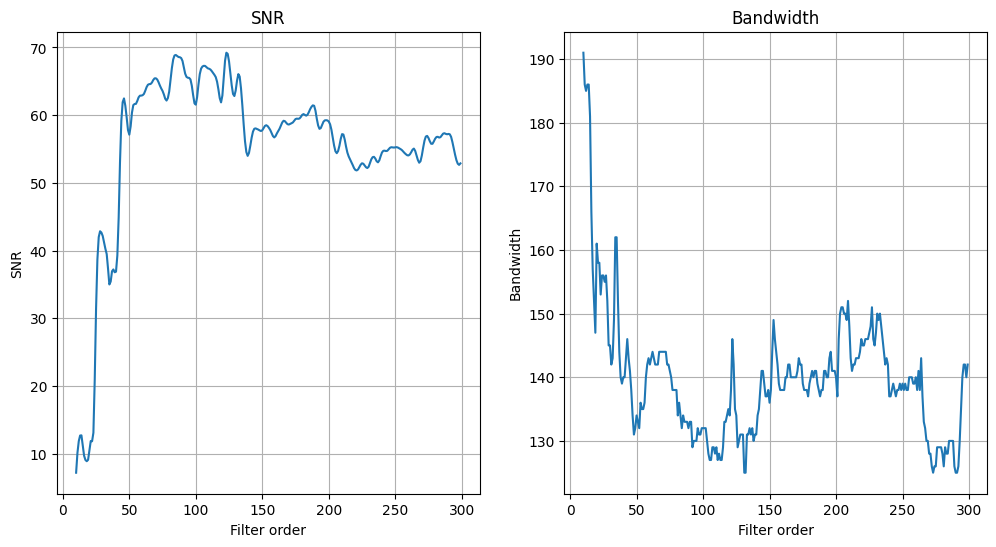
\includegraphics[width=1.0\columnwidth]{images/wiener_filter_length.png}
	\end{center}
	\caption{The effect of the number of Wiener filter coefficients on the SNR and signal integrity}
	\label{fig:wiener_filter_length}
\end{figure}

\subsubsection{Adaptive Wiener filter}

\textcolot{red}{Todo: write this}

\subsection{Results}
Each filter will be tested using two metrics: SNR (eq \ref{eq:rms}) and signal integrity (definition of this will be given shortly). All filters are linear time invariant which means the superposition principle can be used to simplify SNR calculations \cite{linear_systems_theory}. The superposition principle simply states that filtering the sum of two signals is the same as filtering the signals individually and adding the results. An illustration of this can be seen in \ref{fig:filter_process}. A sample of noise data and a sample of EMG data is taken from \ref{fig:sEMG_signal_example} where noise is taken to be 0-2s and signal is taken to be 5-\SI{7}{\second}. The RMS of the filtered signal is divided by the RMS of the filtered noise to create a signal to noise ratio.

\begin{figure}[h!t]
	\begin{center}
		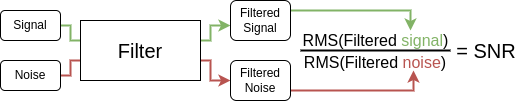
\includegraphics[width=1.0\columnwidth]{images/filter_process.png}
	\end{center}
	\caption{Illustration of testing of filters. Signal and noise are passed through the filter invidiually and the SNR is calculated for each filter.}
	\label{fig:filter_process}
\end{figure}

A property that might be of interest is each filters performance in different levels of Maximum Voluntary Contraction (MVC). This allows for insight into how well each filter functions in different levels of signal compared to the environment noise. This was realized by keeping the noise constant, but scaling the signal to different levels (from 1-\SI{100}{\percent}) to simulate different levels of MVC. The SNR of the filtered signal and filtered noise was divided by the reference SNR (SNR of input signal and input noise) to be able to draw a clear conclusion about the filters performance.

\begin{figure}[h!t]
	\begin{center}
		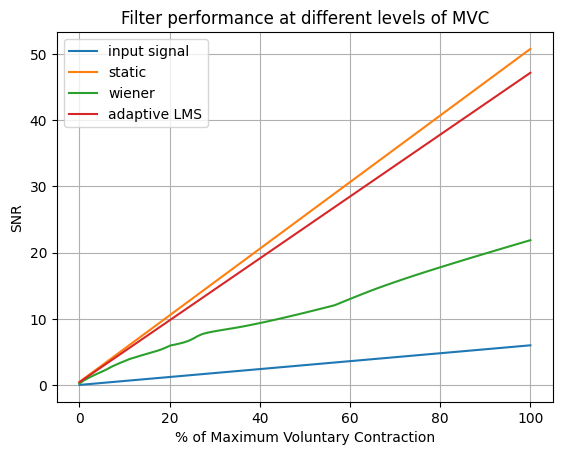
\includegraphics[width=0.7\columnwidth]{images/filter_snr_mvc.png}
	\end{center}
	\caption{The SNR of each filter for different levels of MVC. It can be seen that there is no relation between a filters performance and the degree of contraction.}
	\label{fig:filter_snr_mvc}
\end{figure}

SNR by itself is not a valid metric for judging a filters performance in this scenario. The purpose of improving SNR is the assumption that force can be estimated more accurately from a signal that contains primarily the signal generated by muscle contraction. However, a filter may be able to attenuate the signal and noise in such a way that the SNR is very high, but the signal is attenuated to such a degree that it no longer resembles the original signal that was generated by the muscle contraction. An example of this can be seen in figure \ref{fig:good_snr_bad_integrity}. To account for this, a new metric is introduced called 'Signal integrity', of which the mathematical definition is given in equation \ref{eq:signal_integrity}. By dividing a filters output frequency spectrum by the input frequency spectrum (each frequency component in the before-fft divided by its corresponding after-fft counterpart) it is possible to determine how much the frequency spectrum has changed by the filter. If the resulting value of a frequency after this division is 1, the filter did not attenuate this frequency at all. If the result of this division is 0, then the frequency component has been removed entirely. 

Taking the mean of these values should give an indication of the degree of attenuation that a signal experiences when filtered. Doing this for both the signal and the noise separately, a conclusion can be drawn about how much the frequency spectrum of the noise is attenuated \textit{more} than the frequency spectrum of the signal. 

An ideal filter would not attenuate the frequency spectrum of the signal while completely nullifying the frequency spectrum of the noise. The resulting signal integrity value would be 1. If a filter does not attenuate the signal but neither attenuates the noise, the signal integrity value would be 0. If the filter attenuates the signal more than it attenuates the noise, the signal integrity value would be less than 0.

\begin{equation}
    Filter integrity = \frac{\text{FFT}(sig \;\; after)}{\text{FFT}(sig \;\;  before)} / \frac{\text{FFT}(noise \;\;  after)}{\text{FFT}(noise \;\;  before)}
    \label{eq:signal_integrity}
\end{equation}

\begin{figure}[h!t]
	\begin{center}
		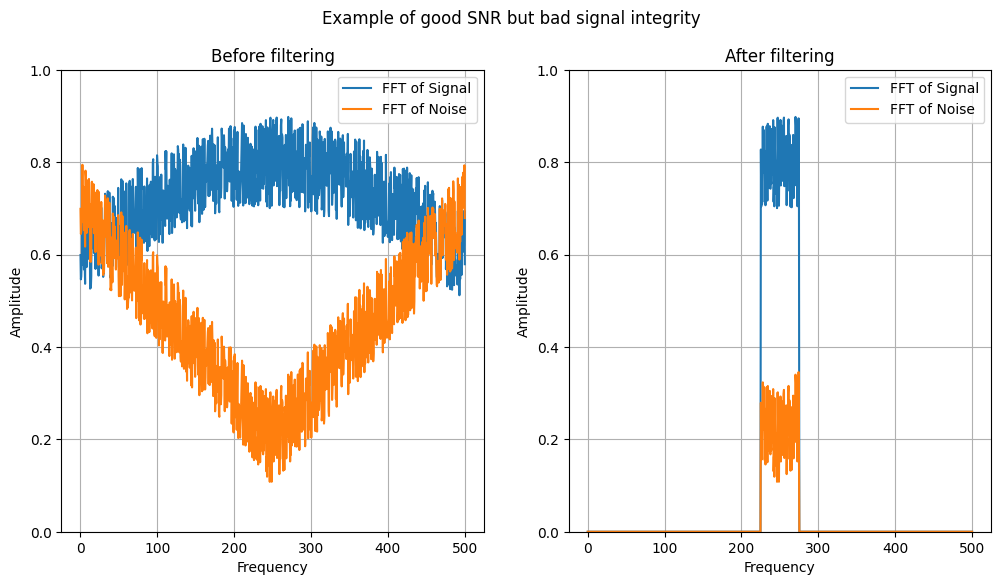
\includegraphics[width=1.0\columnwidth]{images/good_snr_bad_integrity.png}
	\end{center}
	\caption{Example of filtering that results in good SNR but bad signal integrity.}
	\label{fig:good_snr_bad_integrity}
\end{figure}

Again, the signal integrity was calculated for different filters and at different levels of MVC. The results can be seen in figure \ref{fig:filter_signal_integrity_mvc}.

\begin{figure}[h!t]
	\begin{center}
		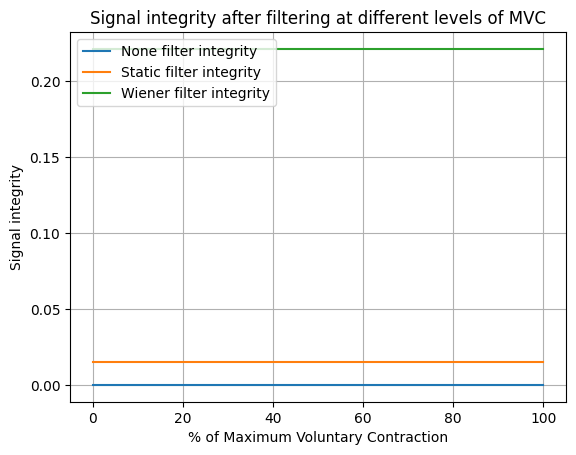
\includegraphics[width=0.7\columnwidth]{images/filter_signal_integrity_mvc.png}
	\end{center}
	\caption{The signal integrity of each filter for different levels of MVC. It can be seen that there is no relation between a filters performance and the degree of contraction}
	\label{fig:filter_signal_integrity_mvc}
\end{figure}

For the static filter a few different variations were tested. Looking at figure \ref{fig:sEMG_fft_signalnoise_example} it can be seen that beside the \SI{50}{\hertz} peak in the noise spectrum there are additional peaks at multiples of \SI{50}{\hertz} (\SI{100}{\hertz}, \SI{150}{\hertz}, etc). Static filters were tested starting from no notch filters (Static 0), and going up to 4 notch filters (Static 4). Static 1 has a single notch filter at \SI{50}{\hertz}, static 2 has a notch at \SI{50}{\hertz} and one at \SI{100}{\hertz}, etc. The resulting metrics can be seen in table \ref{tab:static_filter_snr_integrity}.

\begin{table} [h!]
    \begin{tabular}{c|c|c}
        Filter type & SNR & Signal integrity\\
        \hline
        None & 1.0 & 0.0\\
        Static 0 & 2.443 & 0.045\\
        Static 1 & 5.796 & 0.015\\
        Static 2 & 2.426 & 0.03\\
        Static 3 & 2.433 & 0.044\\
        Static 4 & 2.47 & 0.05\\
    \end{tabular}
    \caption{SNR and signal integrity for different static filters.}
    \label{tab:static_filter_snr_integrity}
\end{table}

\section{Envelope estimation}
The construction of different envelope estimation techniques will be discussed in the method section. The metric for testing performance with be discussed in the results section, as well as the results themselves.

\subsection{Method}
\subsubsection{IIR lowpass filter}
A Butterworth filter was used to construct an IIR lowpass filter. The performance of such a lowpass filter is defined by its cut-off frequency and the number of filter coefficients (or the filter order). It was empirically determined that the maximum frequency for switching between total relaxation and maximum voluntary contraction was around \SI{5}{\hertz} and thus the cut-off frequency was varied from \SI{1}{\hertz}-\SI{9}{\hertz}. The filter order was varied from 2-8 because the minimum possible filter order is 2 (a single filter coefficient provides no filtering, just scaling the signal with a constant), and a filter order >8 resulted in unstable behaviour. A plot of the frequency response of the IIR Butterworth filter can be seen in figure \ref{fig:iir_frequencyresponse_coefficients}. The filters are achieved as a numerator/denominator sequence. Since the purpose of this filter is real-time envelope detection, it was applied using scipy's lfilter since as that is causal forward-in-time filtering only.


\begin{figure}[h!t]
	\begin{center}
		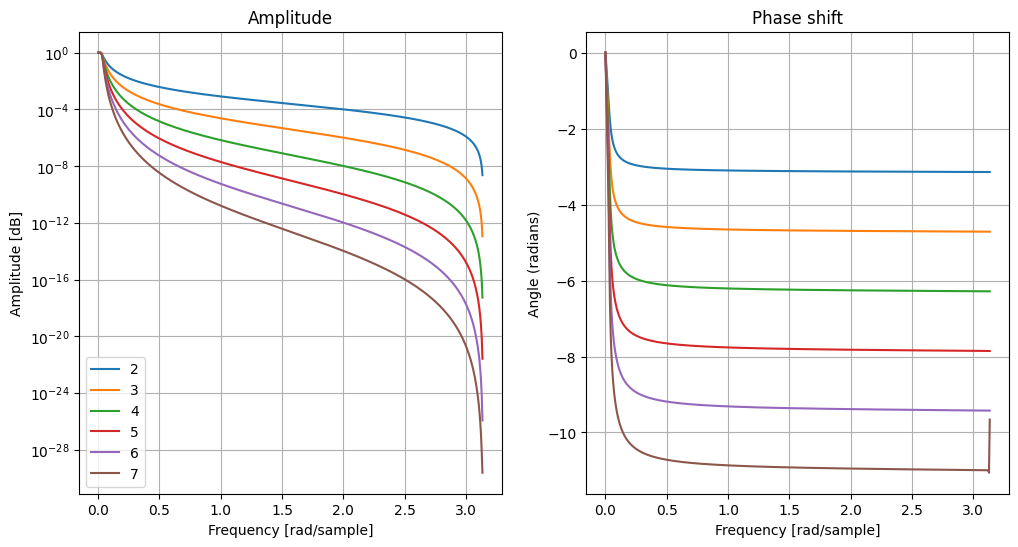
\includegraphics[width=1.0\columnwidth]{images/iir_frequencyresponse_coefficients.png}
	\end{center}
	\caption{Frequency response of IIR Butterworth filter of different lengths. The cut-off frequency was set to 5Hz.}
	\label{fig:iir_frequencyresponse_coefficients}
\end{figure}

\subsubsection{Moving average}
The moving average filter only depends on the length of the filter, figure \ref{fig:movingaverage_frequencyresponse_coefficients} depicts the frequency behaviour of the moving average filter of different lengths. The range of values that are tested is chosen arbitrarily, but large enough to cover general use cases.

\begin{figure}[h!t]
	\begin{center}
		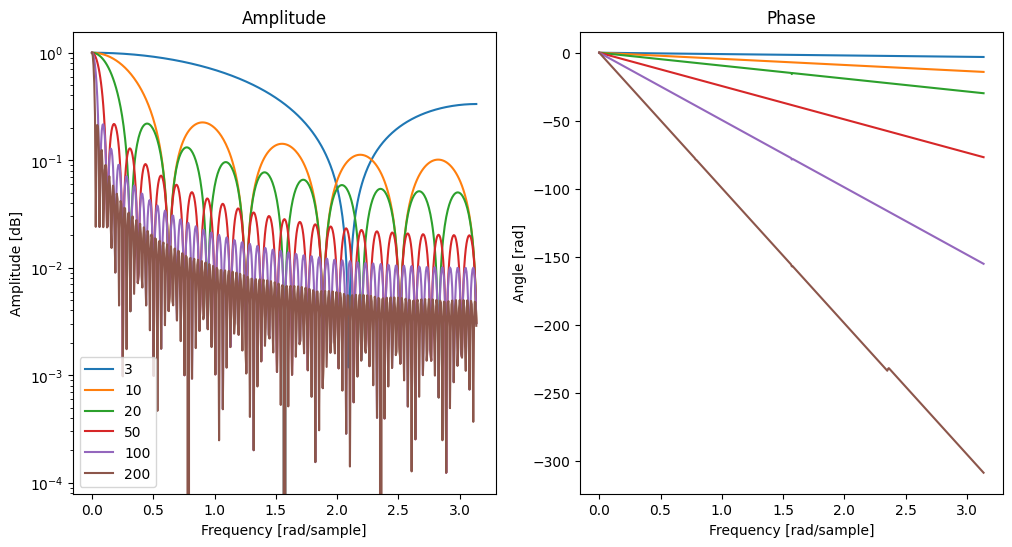
\includegraphics[width=1.0\columnwidth]{images/movingaverage_frequencyresponse_coefficients.png}
	\end{center}
	\caption{Frequency response of moving average filter of different lengths. The coefficients of the moving average filters are 1/length of filter.}
	\label{fig:movingaverage_frequencyresponse_coefficients}
\end{figure}

\subsubsection{Root mean square}
Similar to the moving average filter, the behaviour of the RMS filter is solely determined by the length of the filter. The same range of filter lengths was chosen as for the moving average filter so that the performance could be directly plotted against each other.

\subsection{Results}
There are two seperate metrics that need to be measured when comparing envelope estimation techniques. The first one is how 'fast' a techniques is, and the second is how 'good' the technique is. The first metric gives information about how much the 'detected' signal lags behind the 'true' signal. The second metric is the quality of the envelope estimate when accounting for the lag. 

The lag is detected by calculating the cross-correlation between the true signal and the envelope estimate. Cross-correlation is a metric that determines the similarity between two signals as a function of displacement of one signal relative to another \cite{wiki:cross_correlation}. Since the 'true' signal and the estimated signal are most similar when their displacement equals the lag, a detectable peak is formed in the cross correlation function. The left subplot in figure \ref{fig:envelope_estimation_method} displays a 'true' signal (measured force), and a simulated estimation of this signal (estimated force) that lags behind the true signal. The cross-correlation is also plotted that has a peak at \SI{100}{\milli\second}, which is the exact amount of lag between the two signals. The right subplot shows the two signals where the estimated signal has shifted to account for the lag. At this point the error can be determined by subtracting the true signal from the estimated signal, and the root-mean-square-error can be calculated. 

\begin{figure}[h!t]
	\begin{center}
		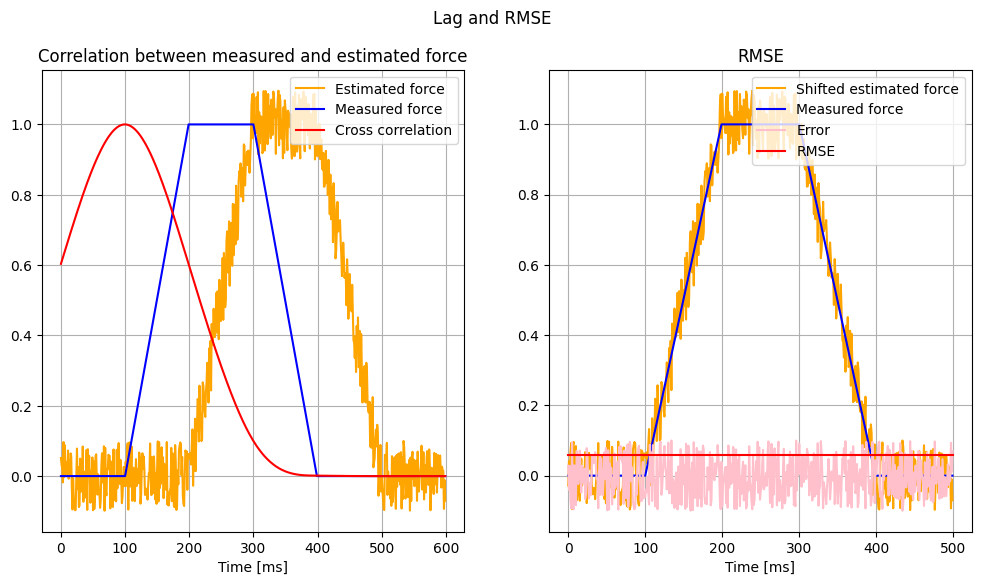
\includegraphics[width=1.0\columnwidth]{images/envelope_estimation_method.png}
	\end{center}
	\caption{Illustration of method for judging envelope estimation}
	\label{fig:envelope_estimation_method}
\end{figure}

The input signal was generated to be gaussian white noise since it has signal properties close to that of an sEMG signal, and is multiplied with a modulation that can be seen in the left subplot of figure \ref{fig:envelope_detection}. The envelope detection techniques are applied onto the input signal and the results are plotted in the right subplot of figure \ref{fig:envelope_detection}.

\begin{figure}[h!t]
	\begin{center}
		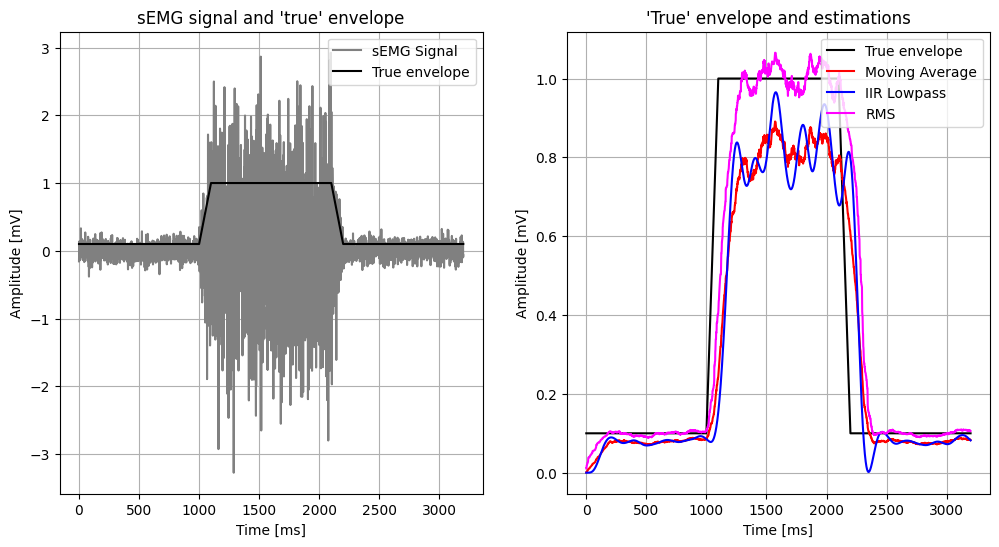
\includegraphics[width=1.0\columnwidth]{images/envelope_detection.png}
	\end{center}
	\caption{Left: Input signal and 'true' envelope'. Right: Envelope detection using different techniques to illustrate difference in behaviour}
	\label{fig:envelope_detection}
\end{figure}

To properly evaluate the performance of the envelope detection techniques each method has been tested individually across the range of variables that were described in the previous method section and plotted against the resulting lag and error. The graph describing the performance of the IIR butterworth filter can be seen in figure \ref{fig:lagerror_iir}. The graph describing the performance of the moving average filter and the RMS filter can be seen in figure \ref{fig:lagerror_RMS_MA}.

\begin{figure}[h!t]
	\begin{center}
		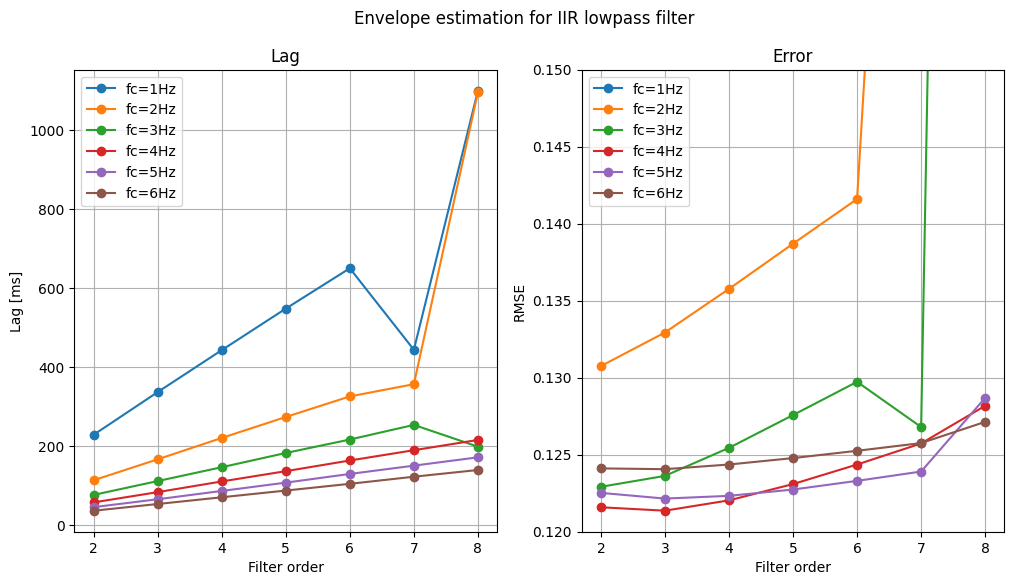
\includegraphics[width=1.0\columnwidth]{images/lagerror_iirfilter.png}
	\end{center}
	\caption{Lag and error of an IIR butterworth filter for different cut-off frequencies and filter lengths. Note that filters with a lower cut-off frequency and high number of filter coefficients become unstable which can be seen in the error-graph for cut-off frequencies \SI{1}{\hertz}-\SI{3}{\hertz}. Additionally, the error in these graphs are all below 0.125. This is caused by the fact that the modulation is between 0 and 1, the error is <1 and the squared error is smaller still. So not the error value, but the \textit{relation between} = error values of different methods is the truly useful information here.}
	\label{fig:lagerror_iir}
\end{figure}

\begin{figure}[h!t]
	\begin{center}
		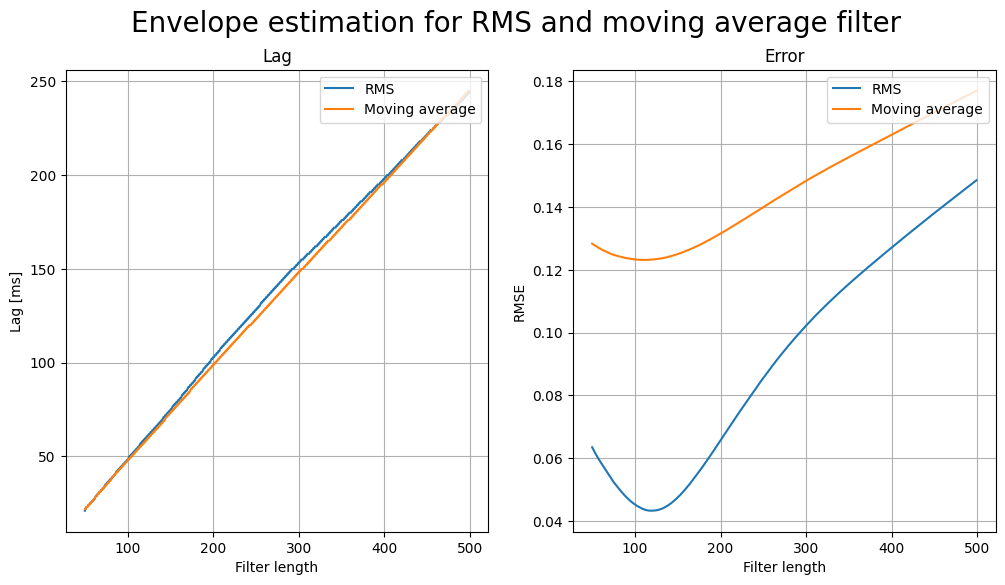
\includegraphics[width=1.0\columnwidth]{images/lagerror_rms_and_MA_filter.png}
	\end{center}
	\caption{Lag and error of RMS filter and moving average filter for different filter lengths}
	\label{fig:lagerror_RMS_MA}
\end{figure}

\section{Force estimation}\label{section:force_estimation}

The measured sEMG signals from antagonistic muscles needs to be combined to form an estimate of the exerted force. Since this calculation is done in a consistent way throughout all measurements this section serves purely to provide some insight into the method of calculation.

The previous step of envelope estimation is used to get a measure of muscle contraction. Exerted force around a joint is simply the difference between how much antagonistic contract. By measuring the sEMG from antagonistic muscles (such as bicep and tricep) and determining their envelope after processing, the estimated force is simply the difference between the two envelopes. However, this method does not directly result in an estimation of force but actually an estimation in the difference of muscle contraction. To correlate the difference in muscle contraction from antagonistic muscles to the exerted force, the muscle contraction needs to be scaled. As previously mentioned, a linear relation between sEMG and force will be assumed \cite{adaptive_filter_dry_electrode} \cite{interpreting_muscle_function_from_emg}. In figure \ref{fig:force_simulation} it is shown how the exerted force is estimated from simulated bicep and tricep sEMG. 

\begin{figure}[h!t]
	\begin{center}
		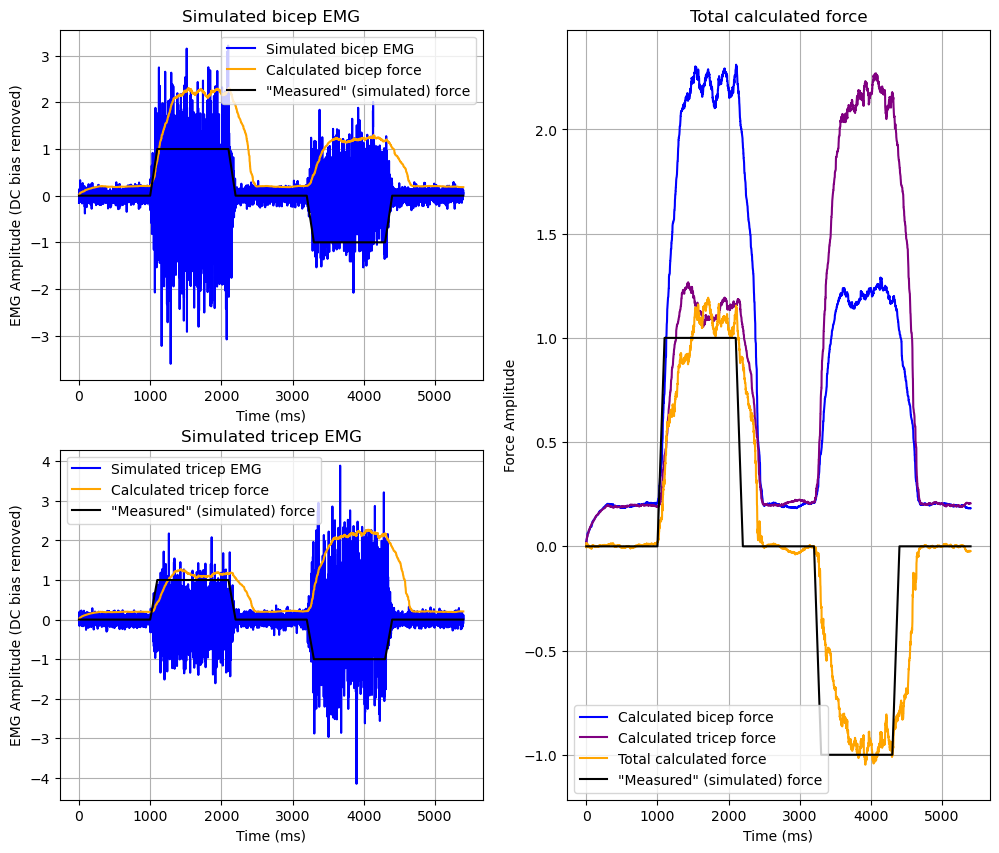
\includegraphics[width=0.7\columnwidth]{images/force_simulation.png}
	\end{center}
	\caption{Process of estimating force from simulated sEMG (random Gaussian noise). The bicep envelope is calculated at the top, notice how during downwards force exertion the bicep still activates but to a lesser degree than during upwards force exertion. The same holds for the tricep in the bottom figure. The subplot on the right shows the envelope of the bicep, tricep, the difference between these two (identical to estimated force assuming linear scaling with factor 1), and the 'measured' force .}
	\label{fig:force_simulation}
\end{figure}

